\chapter{Parallélisation }
Les programmes que nous écrivons sont tous séquentiels, c'est-à-dire que les instructions vont s'exécuter les unes à la suite des autres ce qui engendre des temps d'exécution conséquents pour les programmes lourds comme pour le calcul des forces gravitationnelles.
La parallélisation ou programmation parallèle est un moyen d'optimiser notre programme et réduire son temps d'exécution. 
Elle consiste à effectuer des tâches de manière simultanées. Ainsi, un programme parallèle pourra exécuter en même temps des processus défini de manière séquentielle.\\

Ici, nous nous intéressons à la parallélisation multi-threads à mémoire partagée à travers l'interface de programmation (API) OpenMP.

Un thread ou processus léger est un fil d'exécution qui constitue un processus et permet donc d'exécuter du code machine dans le processeur. Ainsi, l'exécution d'un programme lance un processus qui va ensuite lancer plusieurs threads.


\begin{center}
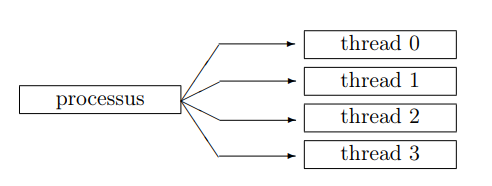
\includegraphics[scale=0.8]{images/process_thread.png}
\captionof{figure}{Processus et threads}
\label{fig4}
\end{center} 

Dans le cas d'un programme séquentiel, seul le thread 0 effectuera une tâche tandis qu'en programmation parallèle, ils seront plusieurs.

La particularité des threads est qu'ils partagent la même zone mémoire ce qui permet donc la parallélisation à condition que le programme soit "compatible".

\section{Fonctionnement d'OpenMP}
\subsection{Principe}
OpenMp est une interface pour la parallélisation multi-threads à mémoire partagée. Elle permet simplement, à partir d'instruction similaire à celle du pré-processeur de paralléliser un programme.

Le principe est ici de paralléliser des blocs d'instructions comme des boucles. Ainsi, un programme utilisant OpenMp est constituée de région séquentielle et de région parallèle. En début de région parallèle, le thread 0 lance alors la création de nouveaux threads.

Il est important de préciser que pour avoir une parallélisation efficace, il est nécessaire d'éviter de refaire des calculs inutiles et de s'assurer que chaque tâches peut s'effectuer sans déranger les autres notamment au niveau de la mémoire partagée.

\subsection{Directives et fonctions importantes}
OpenMp est une API simple à utiliser, il est donc possible de paralléliser un code à partir d'instruction simples.

La plus importante et intéressante pour nous est celle permettant de paralléliser une boucle for :

\begin{lstlisting}
#pragma omp parallel for
\end{lstlisting}

Voici également des fonctions qui peuvent s'avérer utiles:

\begin{lstlisting}
omp_get_num_threads() //retourne le nombre total de threads utilisés
omp_set_num_threads(int) // spécifie un nombre de thread dans une région parallèle
omp_get_thread_num() // retourne le numéro du thread courant
\end{lstlisting}

\section{Application à notre programme de résolution du problème à N-corps}

Dans notre cas, les processus les plus lourds sont les calculs de forces gravitationnelle et la création de l'arbre, c'est donc ceux-ci que nous allons paralléliser.

\begin{itemize}
\item La construction de l'arbre : les particules peuvent être ajoutées parallèlement cependant, il est possible d'obtenir des problèmes de synchronisation, il est donc intéressant de vérifier si la parallélisation effective.

\item Le calcul des forces : les calculs intermédiaires (distances...) sont stockés dans des variables temporaires ce qui facilite la parallélisation.
\end{itemize}

